\documentclass[20pt]{article}
\usepackage{hyperref}

\usepackage[a4paper]{geometry}
\geometry{left = 4.0cm, right = 4.0cm, top = 4cm, bottom = 4cm}


\usepackage{fancyhdr}
\usepackage{algorithm}
\usepackage{amsmath}
\usepackage{amsthm}
\usepackage{amssymb}
\usepackage{amsfonts}
\usepackage{graphicx}
\usepackage{braket}
\usepackage{fontsize}
\usepackage{multicol}
\usepackage{mdframed}
\usepackage{multirow}
\usepackage{wrapfig}
\usepackage{booktabs}
\usepackage{circuitikz}
\usepackage{array}
\usepackage{pgfplots}
\usepackage{tikz-cd}
\usepackage[capitalise]{cleveref}
\usepackage{graphicx}
\usepackage{listings}
\usepackage{hyperref}

\usepackage{biblatex}
\addbibresource{ref.bib}
\usepackage[english]{babel}


\theoremstyle{definition}
\newmdtheoremenv[]{definition}{\hspace{2em}Definition}[section]
\newmdtheoremenv[]{theorem}{\hspace{2em}Theorem}[section]
\newmdtheoremenv[]{prop}{\hspace{2em}Proposition}[section]
\newmdtheoremenv[]{corollary}{\hspace{2em}Corollary}[section]
\newmdtheoremenv[]{example}{\hspace{2em}Example}[section]
\newmdtheoremenv[]{lemma}{\hspace{2em}Lemma}[section]

\usepackage[dvipsnames]{xcolor}
\definecolor{codegreen}{rgb}{0,0.6,0}
\definecolor{codegray}{rgb}{0.5,0.5,0.5}
\definecolor{codepurple}{rgb}{0.58,0,0.82}
\definecolor{backcolour}{rgb}{0.95,0.95,0.92}
% Definig a custom style:
\lstdefinestyle{mystyle}{
    backgroundcolor=\color{backcolour},   
    commentstyle=\color{codepurple},
    keywordstyle=\color{NavyBlue},
    numberstyle=\tiny\color{codegray},
    stringstyle=\color{codepurple},
    basicstyle=\ttfamily\footnotesize\bfseries,
    breakatwhitespace=false,         
    breaklines=true,                 
    captionpos=t,                    
    keepspaces=true,                 
    numbers=left,                    
    numbersep=5pt,                  
    showspaces=false,                
    showstringspaces=false,
    showtabs=false,                  
    tabsize=2
}
% -- Setting up the custom style:
\lstset{style=mystyle}

\title{\textbf{MCM Thesis}}
\author{ABC}


\begin{document}
\maketitle

\begin{abstract}
	This is the abstract.
\end{abstract}

\newpage

\tableofcontents
\newpage

\section  {Introduction} \ 

This is an introduction \cite{urban} \cite{barringer2020worldwide} \cite{horton2021mcm}
\section  {Assumptions} \ 

Our assumptions are:

\begin{itemize}
	\item \textbf{item 1} 
	\item \textbf{item 2}
	\item \textbf{item 3}
\end{itemize}

\section  {Our Model} \ 

\begin{table}[h!]
\centering
\begin{tabular}{|c|c c c|} 
 \hline
 Col1 & Col2 & Col2 & Col3 \\ [0.5ex] 
 \hline
 1 & 6 & 87837 & 787 \\ 
 2 & 7 & 78 & 5415 \\
 3 & 545 & 778 & 7507 \\
 4 & 545 & 18744 & 7560 \\
 5 & 88 & 788 & 6344 \\ [1ex] 
 \hline
\end{tabular}
\caption{Table to test captions and labels.}
\label{tab:1}
\end{table}

From \cref{tab:1} the result is clear.


\section {Sensitivity Analysis} \ 


To test the robusness of our solution, we used statistical data (See appendix) to generate random sequences of $W_{d,t}$. By gradually increasing the standard diviation of generated sequence, we evaluate how our solution perform under realistic fluctuations of trash generation. The results are showed in \cref{fig:ttdsen} 

		The generation is achieved by letting:

		\begin{align}
			W_{d,t} \sim \mathcal{N}(m_d, \sigma_d^2)
		\end{align}

		Where $ m_d, \sigma_d^2$ are determined using statistical tonnage data.


\begin{figure}[H]
	\centering
	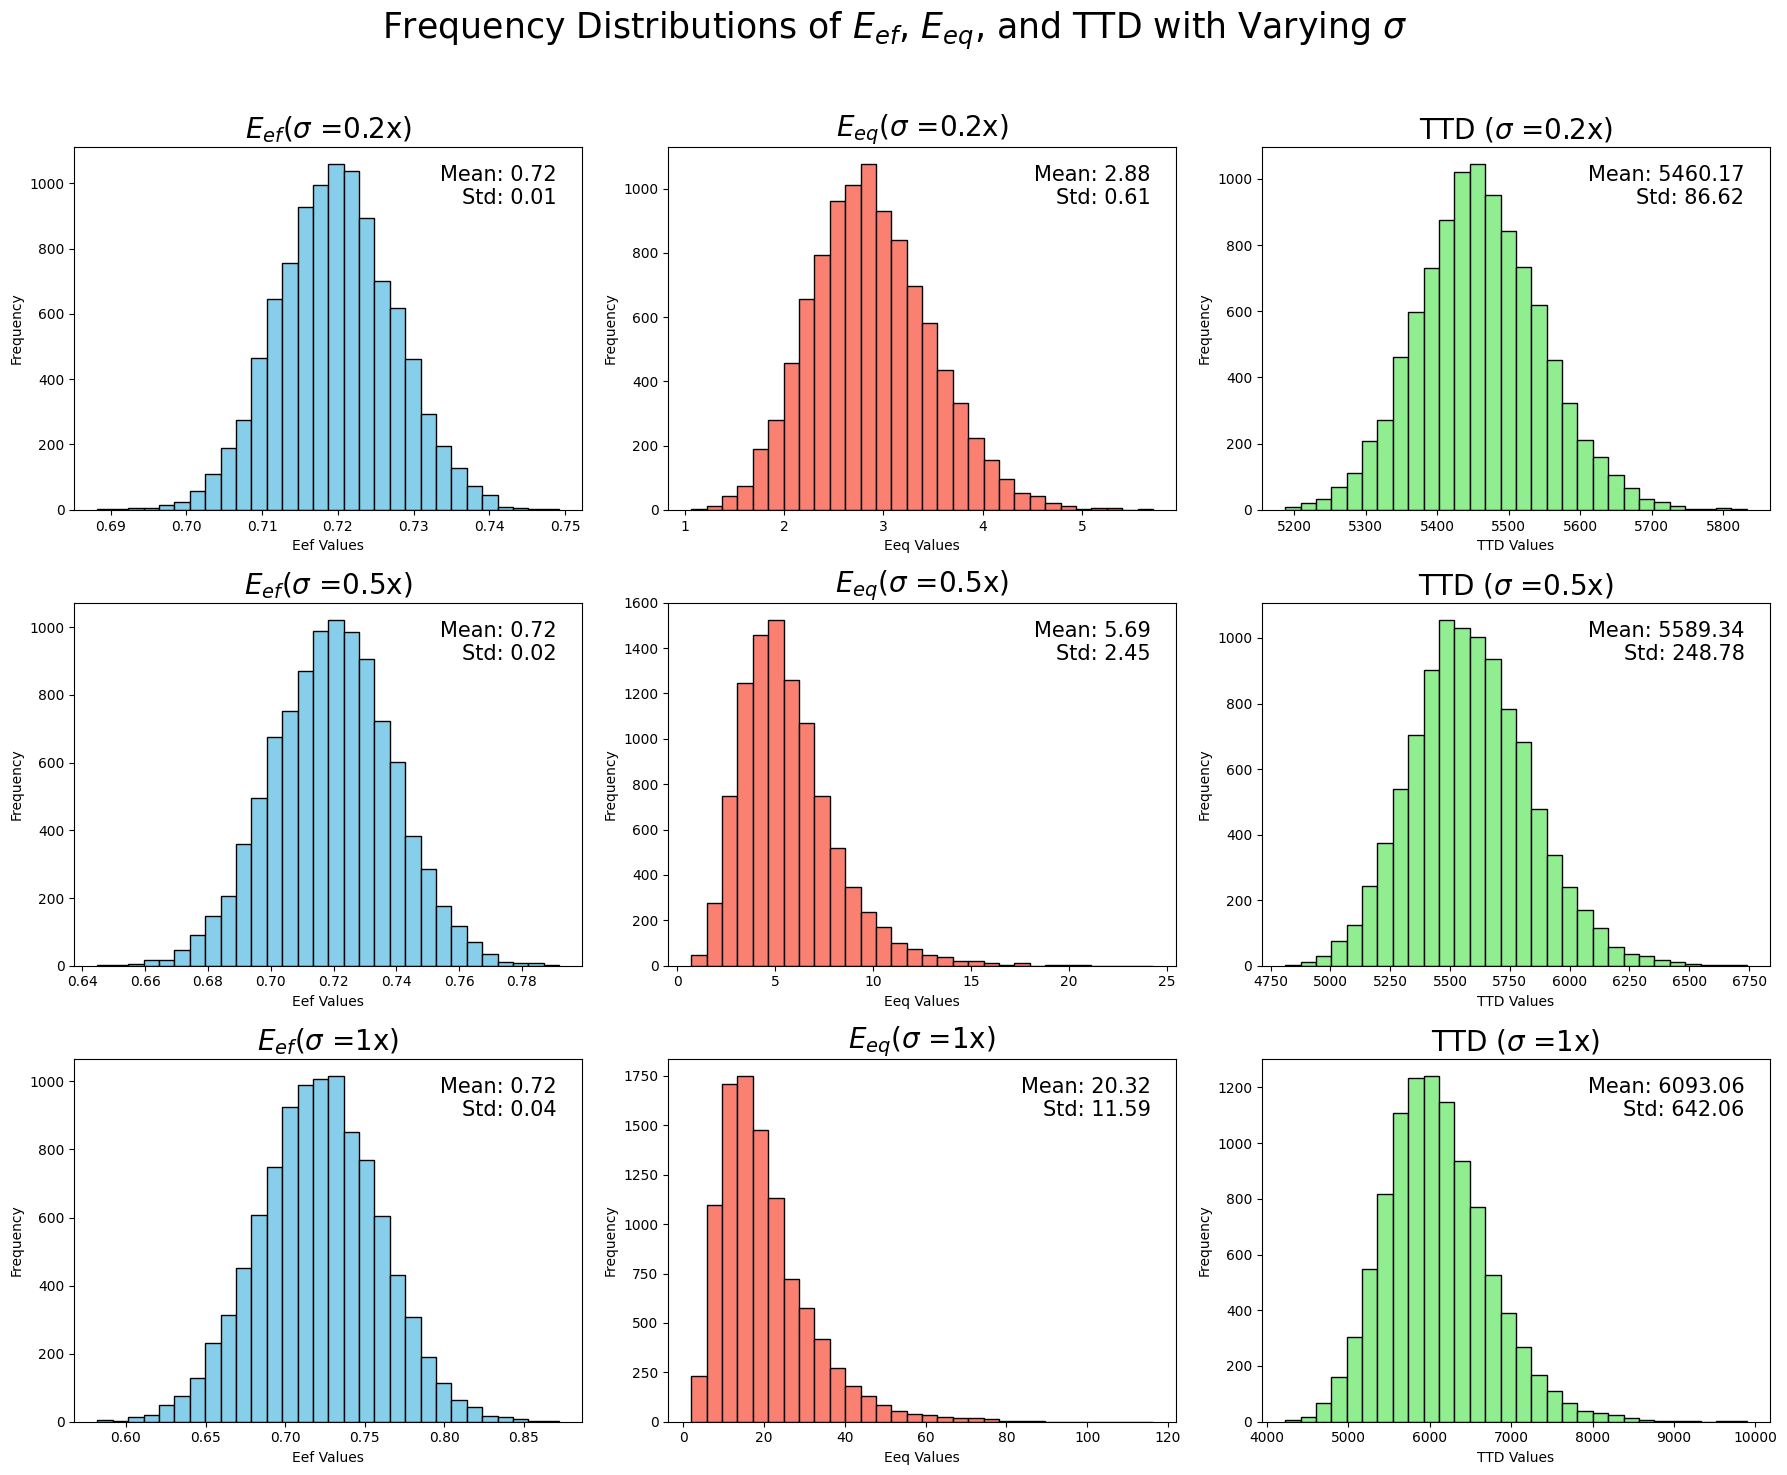
\includegraphics[width=1\textwidth]{figures/sen.png}
	\caption{Sensitivity analysis of the TTD model. We generated 10,000 sets of $ W_{d,t}$ and tested how our solution perform. Where $ \sigma = 0.2x$ denotes $ \sigma = 0.2 \times \sigma_s$, where $ \sigma$ is the standard diviation parameter of the random sequence generation, and $ \sigma_s$ is the statistical value from real world data. 
	From the result we can see that the mean of $ E_{ef} $ and $ TTD$ are not sensitive to the flutuations of trash generation(where $ E_{ef}$ retained it's mean and $ TTD$ has an 10 \% increase). While the mean of $ E_{eq}$ increased drastically when the trasit twords real world data happens. This indicates that in real world sanarios, we are not likely to achieve the desired equity of service.   }
	\label{fig:ttdsen}
\end{figure}


\section  {Conclusion} \ 

\begin{figure}[h]
	\centering
	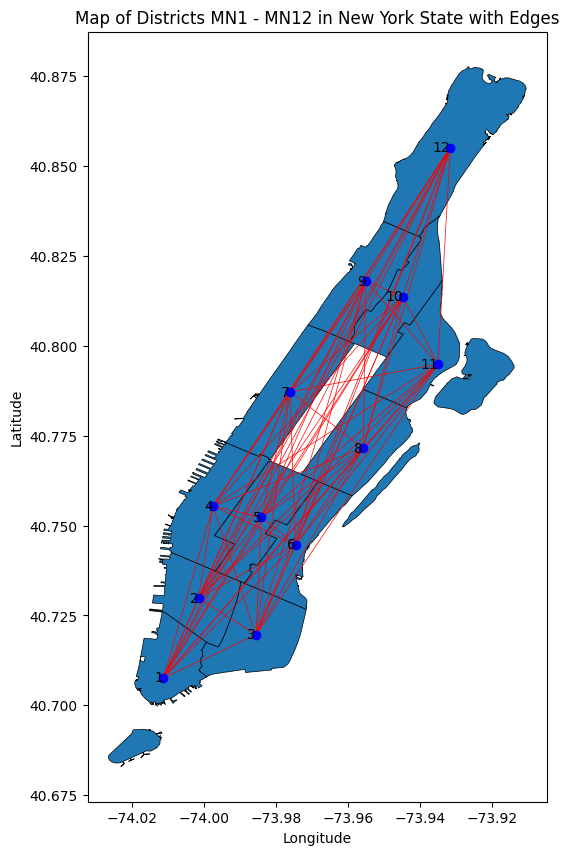
\includegraphics[width=1\textwidth]{figures/graph.png}
	\caption{Visualization of the function}
	\label{fig:sinexp}
\end{figure}

From \cref{fig:sinexp} the result is clear.

\section  {Future Work} \ 

\begin{align}
	E = mc^2 \label{eq:1}
\end{align}
\cref{eq:1}

To account for how long trash stayed at the residency uncollected, we introduce the number $ TTD$ (which stands for total trash delay). Assume we have a schedule for trash collection and we know how much trash is generated each day, then for each district and time $ t$, we can calculate the amount of uncollected trash at time $ t$, denoted by a function $ T(t)$. Given this function, it is natural to quantify the severity of trash delation by the integral:

\begin{align}
	TTD = \int_{t_1}^{t_2} T(t) dt \label{eq:ttd}
\end{align}

Where $ t_1,t_2$ are the start and end times. If all trash are collected immediately once they are generated, then $ T(t) = 0$ for all $ t$ and $ TTD = 0$. While if we collect all trash at once at time $ t_2$ gives a positive $ TTD$ (since if we do not collect any trash in the time interval $ [t_1,t_2]$, then $ T(t)$ is increasing). Both schedules of trash collection 


Since in our problem the time divided into 7 days, the total $ TTD$ for a district is calculated by:


\begin{align}
\sum_{d = 1}^{7} T_d	
\end{align}

\newpage

\section  {Appendix} \ 
\begin{lstlisting}[language=Python, caption=Python example]
import numpy as np
    
def incmatrix(genl1,genl2):
    m = len(genl1)
    n = len(genl2)
    M = None #to become the incidence matrix
    VT = np.zeros((n*m,1), int)  #dummy variable
    
    #compute the bitwise xor matrix
    M1 = bitxormatrix(genl1)
    M2 = np.triu(bitxormatrix(genl2),1) 

    for i in range(m-1):
        for j in range(i+1, m):
            [r,c] = np.where(M2 == M1[i,j])
            for k in range(len(r)):
                VT[(i)*n + r[k]] = 1;
                VT[(i)*n + c[k]] = 1;
                VT[(j)*n + r[k]] = 1;
                VT[(j)*n + c[k]] = 1;
                
                if M is None:
                    M = np.copy(VT)
                else:
                    M = np.concatenate((M, VT), 1)
                
                VT = np.zeros((n*m,1), int)
    
    return M
\end{lstlisting}

\newpage
\printbibliography

\end{document}
